\documentclass[12pt]{article}
\usepackage[utf8]{inputenc}
\usepackage[a4paper, top=2cm, bottom=2cm, left=2cm, right=2cm]{geometry}
\usepackage[T1]{fontenc}
\usepackage[brazilian]{babel}
\usepackage{amsmath, amssymb, amsthm,dsfont}
\usepackage{enumitem}
\usepackage{booktabs}
\usepackage{caption}
\usepackage{graphicx} % needed for images
\usepackage{bm} % para vetor em negrito \bm{x}

\begin{document}

\section*{Atividade 2 -- Regressão}
Aluno: Marcelo Huang\\

\textbf{Enunciado:}  

\subsection*{Descrição}

Nesta atividade, será realizada a simulação de um conjunto de dados a partir de 
um modelo de regressão linear simples com parâmetros 
conhecidos. A partir desses dados, serão conduzidos 
procedimentos de inferência estatística, incluindo o 
teste de hipóteses para o coeficiente angular e a construção 
de intervalos de confiança, além da análise do 
efeito da centralização da variável explicativa sobre 
os parâmetros do modelo. E alguns itens extras adcionados posteriormente.

\subsection*{Itens:}

\textbf{1.a) Simule um conjunto de dados com n pares ($Y_i,X_i$), 
e ajuste o modelo de regressão linear simples.} \\
O modelo considerado é:
\[
Y_i = \beta_0 + \beta_1 X_i + \varepsilon_i
\]
onde $\varepsilon_i \sim N( 0 , \sigma^2 )$, independentes e identicamente distribuídos.
\\
Foi gerado um conjunto de dados com $n = 25$ observações.


A covariável  $X_i$  foi simulada a partir de uma distribuição uniforme no intervalo [10, 20]  (usando a função "runif" do R), 
enquanto o erro aleatório $\varepsilon_i$  foi gerado a partir de uma distribuição normal 
com média zero e desvio padrão igual a 5 ("rnorm(n, mean = 0, sd = 5)").
\\
Atribuindo valores dos parâmetros: $\beta_0 = 16 $ e $\beta_1 = 5$
\\
A variável resposta  $Y_i$  foi então construída de acordo com o modelo especificado.

\begin{figure}[htbp]
\centering
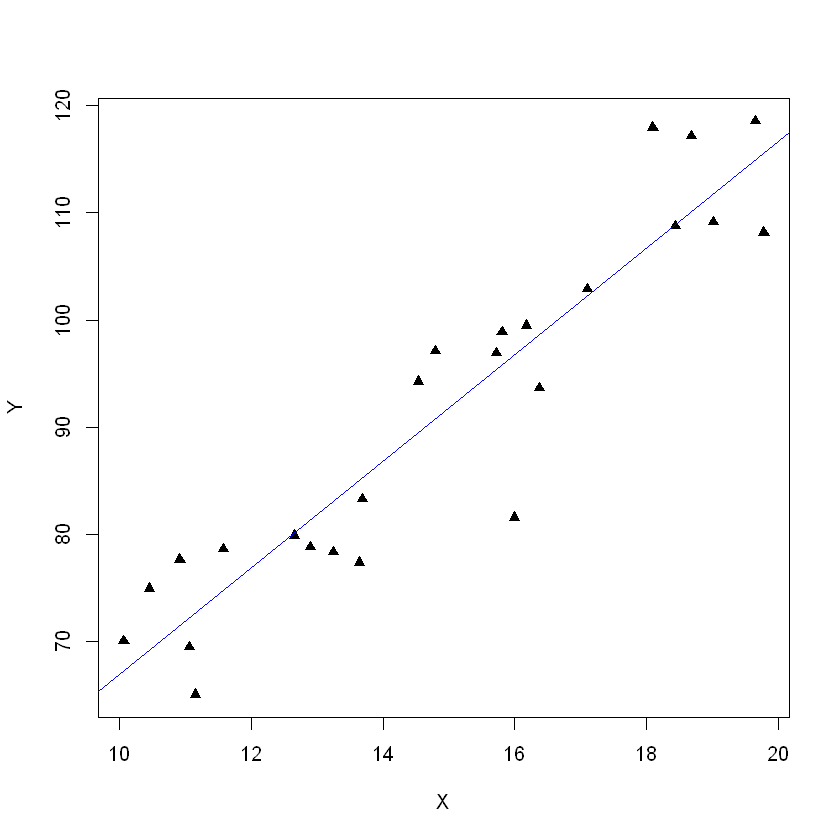
\includegraphics[width=0.5\linewidth]{plot dispersão.png}
\caption{Gráfico de dispersão}
\end{figure}

\begin{table}[htbp]
\centering
\begin{tabular}{lrrr}
\toprule
Os $\beta$'s  & Valor estimado & t  & $Pr(>|t|)$ \\
\midrule
{$\hat{\beta_0}$} & 17,15 & 2,83 & 9.4e-03 \\
{$\hat{\beta_1}$} & 4.97 & 12,47 & 1.02e-11 \\

\bottomrule
\end{tabular}
\caption{Resultados sobre estimadores}
\end{table}

Foi ajustado um modelo de regressão linear simples para avaliar a relação entre $X$ e $Y$.

As estimações foram:  $\hat{\beta_0} = 17.15 $ $\hat{\beta_1}  = 4,97$

---
\textbf{1.b) Teste as hipóteses: }

\[
H_0: \beta_1 = 0 
\]
\[
H_1: \beta_1 \neq 0
\]
\\
Sobre o $\beta_1$, a estatística usada para fazer o teste é 
$t =\frac{\hat{\beta_1} - \beta_1}{EP(\hat{\beta_1})} 
= \frac{\hat{\beta_1} - \beta_1}{\sqrt{MSE/\sum (X_i-\bar{X})^2}}$, 
e essa estatística sob $H_0$ segue uma distribuição $t$ de student com n-2 
graus de liberdade.
\\
A partir dos resultados do teste feito acima, 
observa-se que o coeficiente associado a $X$ é 
estatisticamente significativo, com valor-p (1.02e-11) 
próximo de zero, .

Dessa forma, rejeitamos $H_0$, há evidência de que $\beta_1 \neq 0$, 
indicando uma relação linear entre $X$ e $Y$ no range 
de [10; 20].
\\

\textbf{c) Determine um intervalo de 
confiança para $\beta_1$ Interprete o intervalo}
\\
\begin{table}[htbp]
\centering
\begin{tabular}{lrrr}
\toprule
Intervalo de confiança para Os $\beta$'s & 2.5\%  & 97.5\% \\
\midrule
{$\beta_0$}  & 4.63 & 29.67\\
{$\beta_1$}  & 4.15 & 5.80 \\

\bottomrule
\end{tabular}
\caption{Intervalos de Confiança}
\end{table}

Pela tabela 2, intervalo de confiança de 95\% para $\beta_1$, 
dado por [4.15; 5.8] não contém o valor zero, 
o que evidencia que o coeficiente de 
inclinação $\beta_1$ é diferente de zero e isso indica que, 
em média, um aumento unitário em $X$ 
está associado a um aumento entre 4.15 e 5.8 unidades 
em $Y$.

Além disso, note que o intervalo contém o 
valor verdadeiro utilizado na 
simulação ($\beta_1 = 5$).
\\\\
\textbf{d) Centralize o modelo. 
Ajuste o modelo centralizado. 
Interprete $\beta_0 ^ {*}$ e $\beta_1$. 
Compare os modelos}

$X$ centralizado é dado por:


$X^* = X - \bar{X}$

Assim, $Y_i^* = 
\beta_0^* + \beta_1 X_i^* + 
\varepsilon_i$
onde $\beta_0^* = \beta_0 + \beta_1 \bar{X}$


Em seguida, ajustou-se um novo modelo de regressão 
utilizando $X^*$.

\begin{table}[htbp]
\centering
\begin{tabular}{lrrr}
\toprule
Os $\beta$'s  & Valor estimado & t  & $Pr(>|t|)$ \\
\midrule
{$\hat{\beta_0 ^*}$} & 91.11 & 75.99 & 3.97e-29 \\
{$\hat{\beta_1}$} & 4.97 & 12,47 & 1.02e-11 \\

\bottomrule
\end{tabular}
\caption{Resultados sobre estimadores no modelo centralizado}
\end{table}

\begin{figure}[htbp]
\centering
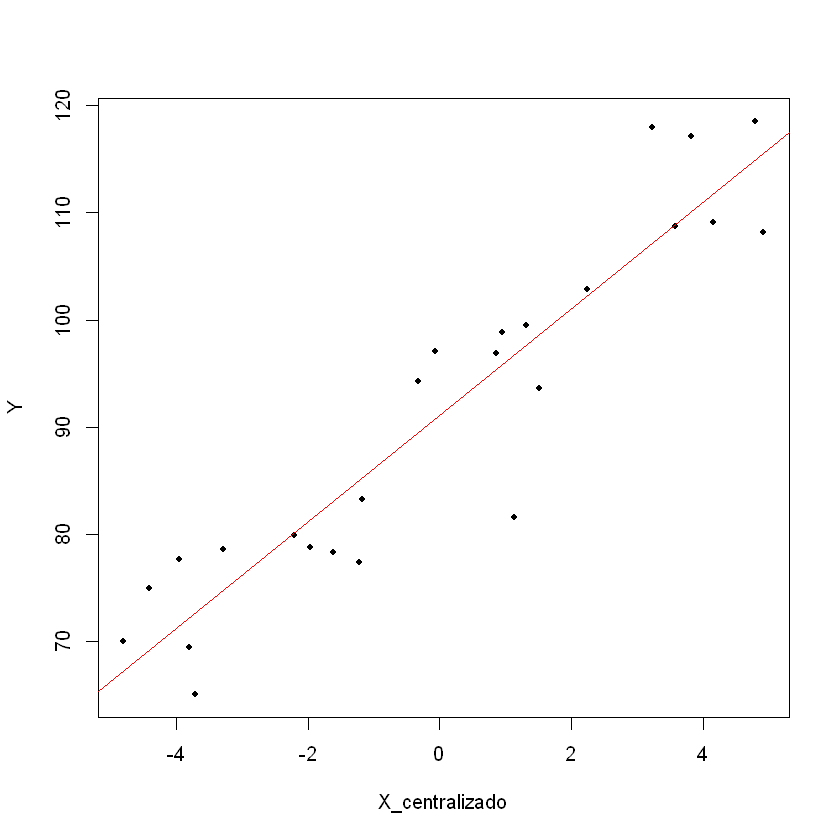
\includegraphics[width=0.5\linewidth]{plot dispersão centralizado.png}
\caption{Gráfico de dispersão (modelo Centralizado)}
\end{figure}
As estimações foram:  $\hat{\beta_0^*} = 91.11 $ e $\hat{\beta_1}  = 4.97$

O intervalo de confiança de 95\% para $\beta_1$ não mudou, 
continua sendo [4.15; 5.8]. E sobre a hipótese $H_0: \beta_1 = 0$, é rejeitada por valor p pequeno. 
Isso é esperado já que o modelo centralizado preserva a 
inferência a $\beta_1$

Comparando os coeficientes dos dois modelos, observa-se que:

- O estimador $\hat{\beta_1}$ para $\beta_1$ e o seu intervalo de confiança permanecem inalterados nos dois modelos.
\\
- O intercepto é modificado ($\beta_0 \neq \beta_0^*$).

No modelo original, o intercepto representa o valor esperado 
de $Y$ quando $X = 0$, o que pode não ter interpretação 
prática, especialmente quando esse valor está fora do 
intervalo observado. 

Enquanto no modelo centralizado, o intercepto ${\beta_0}^*$ 
passa a representar o valor esperado de  $Y$ quando $X = \bar{X}$.
\\
$\hat{\beta_0^*} = 91.11 $: É o valor esperado de $Y_i$ quando é dado que $X_i$ é $\bar{X} $
\\
$\hat{\beta_1} = 4.97$: É epresenta a variação média.
esperada em $Y$ 
quando $X$ aumenta em uma unidade.

Assim, a centralização não altera a inclinação da reta, 
pois a inclinação continua sendo $\beta_1$ (que representa 
a variação esperada em $Y$ associado a um aumento 
unitário em $X$), mas modifica a interpretação do 
intercepto, tornando-o mais informativo quando o 
valor médio de $X$ é relevante.
\begin{figure}[htbp]
\centering
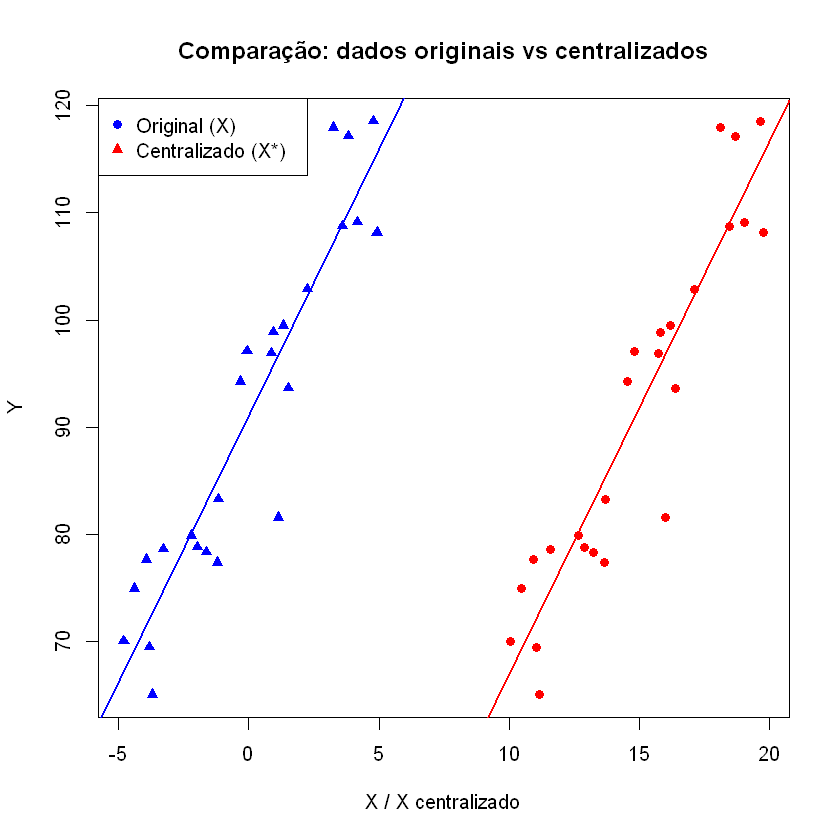
\includegraphics[width=0.3\linewidth]{plot dispersão comparacao.png}
\caption{Comparação: dados originais vs centralizados}
\end{figure}

\textbf{e) Escolha um $X_0$ dentro da amplitude de $X$. 
Encontre um IC 95\% de $Y_0$ esperado desse $X_0$.
Interprete}

Sabemos que $\hat{E(Y_0)} = \hat{Y_0}$, e pelos resultados 
conhecidos, temos uma quantidade pivotal 

$\frac{\hat{Y_0} - E(Y_0)}{\sqrt{MSE/n + (MSE*(X_0-\bar{X})^2) / \sum (X_i-\bar{X})^2}}$
e que segue uma distribuição $t$ de student com n-2 graus de liberdade.
Logo, o intervalo de confiança para $E(Y_0)$ é dado por
\[
\hat{Y_0} \pm t_{n-2, 0.025} \sqrt{MSE\left(\frac{1}{n} + \frac{(X_0 - \bar{X})^2}{\sum_{i=1}^{n} (X_i - \bar{X})^2}\right)}.
\] 
\\
É escolhido um $X_0 = 17.82$, assim o valo de $\hat{Y_0}|X_0 = 17.82$ é 105.836.
e o intervalo de 95 \% de confiança para $E(Y_0)$ é [102.355 , 109.328].
\\
Interpretação:
Com 95\% de confiança, o valor esperado de $Y_0$ quando $X_0$ = 17.82 está entre 102.355 e 109.318 .

\begin{figure}[htbp]
\centering
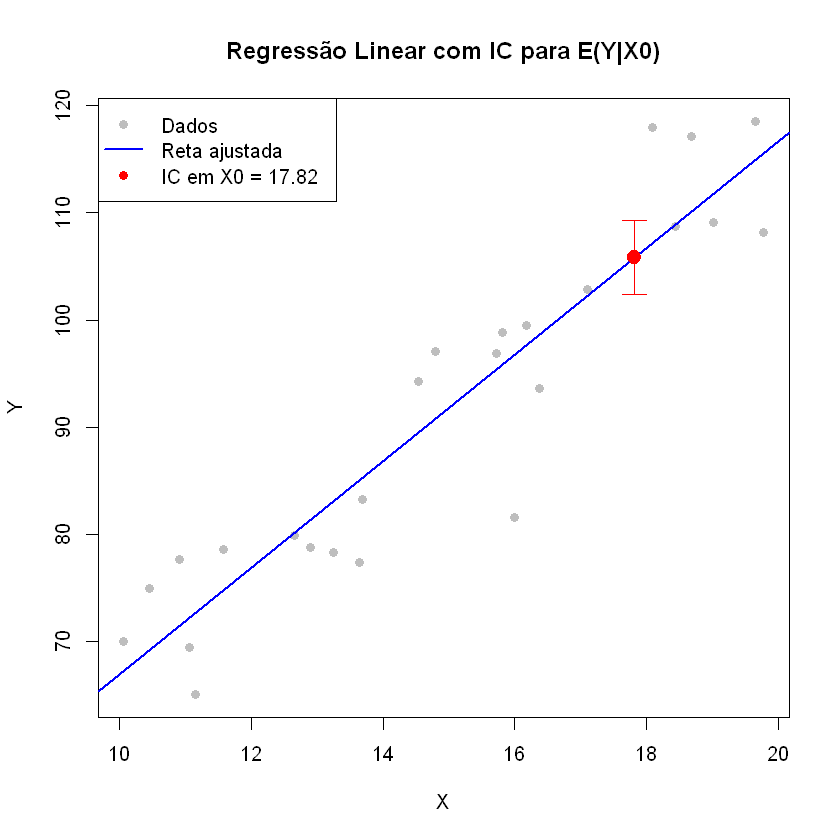
\includegraphics[width=0.5\linewidth]{plot ic E(Y0 dado x0).png}
\caption{}
\end{figure}

\textbf{f) 
Encontre um intervalo de PREDIÇÃO  95\% da variável resposta $Y_0$ desse mesmo $X_0$.
Compare.}
\\
Pelos resultados conhecidos, o intervalo de predição para $Y_0$ é dado por:
\[
\hat{Y_0} \pm t_{n-2, 0.025} \sqrt{MSE\left( \frac{1}{m}+ \frac{1}{n} + \frac{(X_0 - \bar{X})^2}{\sum_{i=1}^{n} (X_i - \bar{X})^2}\right)}.
\] 
(nesse caso $m = 1$ pois só é tirada uma observação de $X_0 = 17.82$)
\\Com o mesmo $X_0 = 17.82$, o intervalo de predição 95 \% para $Y_0$ é [92.96, 118.71]
(espera-se que 95\% das predições futuras estejam dentro desse intervalo).
\\
Comparação: Para o mesmo $X_0$, o intervalo de predição 
é sempre mais amplo que o intervalo de confiança 
para a média. 
\\
O IC quantifica a incerteza 
sobre onde está a média da população; 
o IP quantifica a incerteza sobre onde cairá 
um novo valor individual, 
incluindo a variabilidade aleatória dos erros.\\\\\\\\

\textbf{g) 
Construa uma banda de confiança}
Usando o resultado conhecido sobre Fronteira de Working-Hotelling:

\[
\hat{Y_0} \pm \sqrt{2F^{(0.05)}_{2,\,n-2}} \cdot \sqrt{\hat{Var(\hat{Y_0})}}
\] 

\begin{figure}[htbp]
\centering
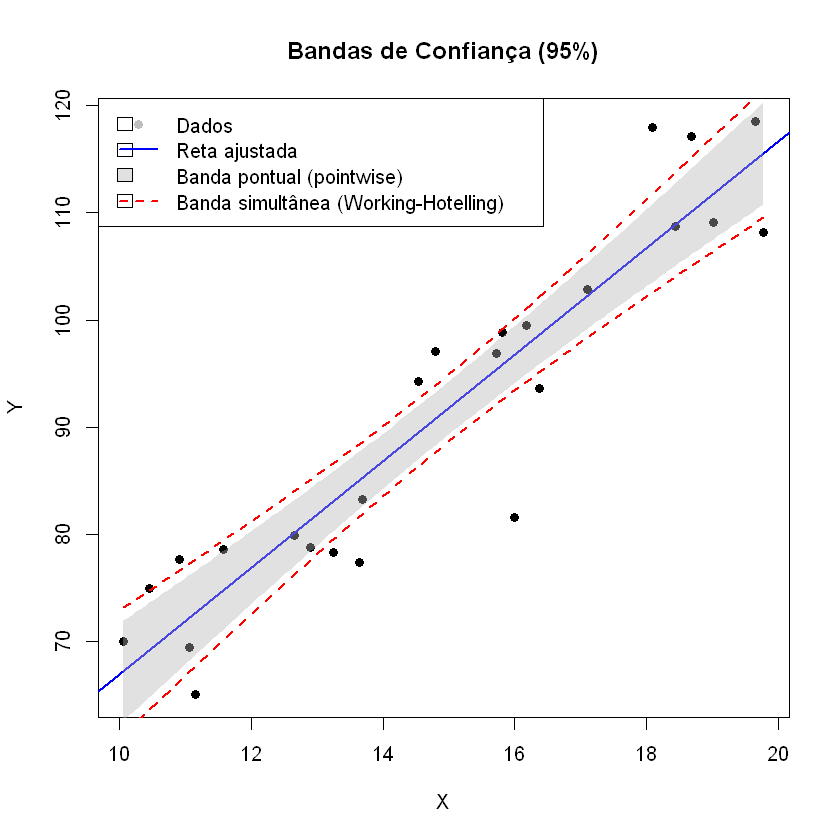
\includegraphics[width=0.5\linewidth]{banda de confianca.png}
\caption{Banda de Confiança}
\end{figure}
A banda vermelha tracejada (figura 5) resultante de Working-Hotelling 
garante, com $(1-\alpha)\%$ de confiança 
(no caso do gráfico $\alpha = 0.05$), 
que toda a reta verdadeira está dentro da 
região para qualquer $X$ no intervalo considerado ([10,20]).

\subsection*{Apêndice}
Códigos usados nessa atividade podem ser acessados via link: 
\\
\texttt{https://github.com/Marcehlin/Atividades-2026\_1}.


\end{document}